\let\negmedspace\undefined
\let\negthickspace\undefined
\documentclass[journal,12pt,onecolumn]{IEEEtran}
\usepackage{cite}
\usepackage{amsmath,amssymb,amsfonts,amsthm}
\usepackage{algorithmic}
\usepackage{amsmath}
\usepackage{graphicx}
\graphicspath{{./figs/}}
\usepackage{textcomp}
\usepackage[utf8]{inputenc}
\usepackage{xcolor}
\usepackage{txfonts}
\usepackage{romannum}
\usepackage{listings}
\usepackage{enumitem}
\usepackage{mathtools}
\usepackage{gensymb}
\usepackage{comment}
\usepackage{caption}
\usepackage[breaklinks=true]{hyperref}
\usepackage{tkz-euclide} 
\usepackage{listings}
\usepackage{gvv}                                        
%\def\inputGnumericTable{}                                     
\usepackage{color}        
\usepackage[utf8]{inputenc}                                     
\usepackage{array}                                            
\usepackage{longtable}         
\usepackage{multicol}                              
\usepackage{calc}                                             
\usepackage{multirow}
\usepackage{multicol}
\usepackage{hhline}                                           
\usepackage{ifthen}                                           
\usepackage{lscape}
\usepackage{tabularx}
\usepackage{array}
\usepackage{float}
\newtheorem{theorem}{Theorem}[section]
\newtheorem{problem}{Problem}
\newtheorem{proposition}{Proposition}[section]
\newtheorem{lemma}{Lemma}[section]
\newtheorem{corollary}[theorem]{Corollary}
\newtheorem{example}{Example}[section]
\newtheorem{definition}[problem]{Definition}
\newcommand{\BEQA}{\begin{eqnarray}}
	\newcommand{\EEQA}{\end{eqnarray}}

\theoremstyle{remark}


\title{\textbf{GATE 2022 ST}}
\author{ EE25BTECH11052 - Shriyansh Kalpesh Chawda}
\begin{document}
	
	\maketitle
	\newpage
	\fbox{\textbf{ {\LARGE Q.1 - Q.5 Carry ONE mark each}}}\\
	\\
	\\
	\\
Q.1 Mr. X speaks \underline{\hspace{2cm}} Japanese \underline{\hspace{2cm}} Chinese. 
\begin{multicols}{4}                                     
\begin{enumerate}[label=(\Alph*)]
		\item neither / or
		\item either / or
		\item neither / nor
		\item also / but
\end{enumerate}
\end{multicols}
\hfill (GATE ST 2022)\\
	\vspace{2em}
	Q.2 A sum of money is to be distributed among P, Q, R and S in the proportion 5:2:4:3 respectively.
	If R gets 1000 more than S, what is the share of Q (in)?
	\begin{multicols}{4}
	\begin{enumerate}[label=(\Alph*)]
		\item 500
		\item 1000
		\item 1500
		\item 2000
	
	\end{enumerate}
\end{multicols}
	\hfill (GATE ST 2022)\\
		\vspace{2em}
Q.3 A trapezium has vertices marked as P, Q, R and S (in that order anticlockwise). The side PQ is parallel to side SR. Further, it is given that: PQ = 11 cm, QR = 4 cm, RS = 6 cm and PS = 3 cm. \\
What is the shortest distance between PQ and SR (in cm)?
\begin{multicols}{4}
	\begin{enumerate}[label=(\Alph*)]
		\item 1.80
		\item 2.40
		\item 4.20
		\item 5.76
		\end{enumerate}
\end{multicols}
\hfill (GATE ST 2022)
		\vspace{2em}
		
Q.4 The figure shows a grid formed by a collection of unit squares. The shaded unit square in the grid represents a hole.
	\begin{figure}[H]
		\centering
		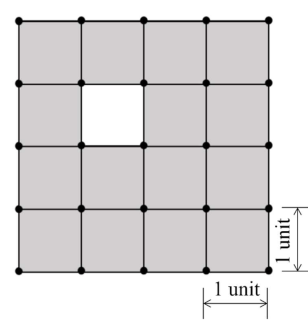
\includegraphics[width=0.3\linewidth]{figs/screenshot001}
		\caption{}
		\label{fig:screenshot001}
	\end{figure}
	\begin{multicols}{4}
	\begin{enumerate}[label=(\Alph*)]
		\item 16
		\item 20
		\item 21
		\item 26
		
	\end{enumerate}
\end{multicols}
\hfill (GATE ST 2022)\\
	\vspace{2em}
Q.5 An art gallery engages a security guard so that the items displayed are protected. The diagram below represents the plan of the gallery where the boundary walls are opaque. The location where the security guard is posted is identified such that all the inner space (shaded region in the plan) of the gallery is within the line of sight of the security guard.\\
If the security guard does not move around the posted location and has a 360° view, which one of the following correctly represents the set of \textbf{ALL} possible locations among the locations P, Q, R and S, where the security guard can be posted to watch over the entire inner space of the gallery?\\
\begin{figure}[H]
		\centering
		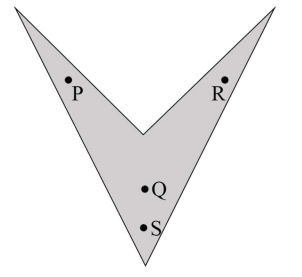
\includegraphics[width=0.4\linewidth]{figs/screenshot002}
		\caption{}
		\label{fig:screenshot002}
\end{figure}
\begin{multicols}{4}
\begin{enumerate}
\item P and Q
\item Q
\item Q and S
\item R and S

\end{enumerate}
\end{multicols}
\hfill (GATE ST 2022)\\
	 \pagebreak
	 \\
	 \fbox{\textbf{ {\LARGE Q.6 - Q.10 Carry two mark each}}}\\
	 \\
	 \\
Q.6 Mosquitoes pose a threat to human health. Controlling mosquitoes using chemicals may have undesired consequences. In Florida, authorities have used genetically modified mosquitoes to control the overall mosquito population. It remains to be seen if this novel approach has unforeseen consequences.
	
Which one of the following is the correct logical inference based on the information in the above passage?
\begin{enumerate}[label=(\Alph*)]
		\item Using chemicals to kill mosquitoes is better than using genetically modified mosquitoes because genetic engineering is dangerous.
		\item Using genetically modified mosquitoes is better than using chemicals to kill mosquitoes because they do not have any side effects.
		\item Both using genetically modified mosquitoes and chemicals have undesired consequences and can be dangerous.
		\item Using chemicals to kill mosquitoes may have undesired consequences but it is not clear if using genetically modified mosquitoes has any negative consequence.
\end{enumerate} 
\hfill (GATE ST 2022)\\
	\vspace{2em}
Q.7 Consider the following inequalities.
\begin{align*}
	\text{(\romannumeral 1)} & \quad 2x - 1 > 7 \\
	\text{(\romannumeral 2)} & \quad 2x - 1 < 1
\end{align*}
Which one of the following expressions below satisfies the above two inequalities?
\begin{multicols}{2} 
	\begin{enumerate}[label=(\Alph*)]
		\item $x \leq -4$
		\item $-4 < x \leq 4$
		\item $4 < x \leq 5$
		\item $x \geq 5$
	\end{enumerate}
\end{multicols}

	 	\vspace{2em}
Q.8 Four points P(0, 1), Q(0, -3), R(-2, -1), and S(2, -1) represent the vertices of a quadrilateral.\\
	 What is the area enclosed by the quadrilateral?[0.5em]
	 \begin{multicols}{4}
	 \begin{enumerate}[label=(\Alph*)]
	 	\item $ 4 $
	 	\item $ 4\sqrt{2} $
	 	\item $ 8 $
	 	\item $ 8\sqrt{2} $
	 
	 \end{enumerate}
	\end{multicols}
		\hfill (GATE ST 2022)\\
	 	\vspace{2em}
Q.9 In a class of five students P, Q, R, S and T, only one student is known to have copied in the exam. The disciplinary committee has investigated the situation and recorded the statements from the students as given below.[0.3em]
	 \textbf{Statement of P}: R has copied in the exam. \\
	 \textbf{Statement of Q}: S has copied in the exam. \\
	 \textbf{Statement of R}: P did not copy in the exam. \\
	 \textbf{Statement of S}: Only one of us is telling the truth. \\
	 \textbf{Statement of T}: R is telling the truth. \\
	 The investigating team had authentic information that S never lies.\\
	 Based on the information given above, the person who has copied in the exam is
	 \begin{multicols}{4}
	 \begin{enumerate}[label=(\Alph*)]
	 	\item R
	 	\item P
	 	\item Q
	 	\item T
	 	
	 \end{enumerate}
	\end{multicols}
	\hfill (GATE ST 2022)\\
	 	\vspace{2em}
Q.10 Consider the following square with the four corners and the center marked as P, Q, R, S and T respectively.\\
Let X, Y and Z represent the following operations: \\
X: rotation of the square by 180 degree with respect to the S-Q axis.\\
Y: rotation of the square by 180 degree with respect to the P-R axis.\\
Z: rotation of the square by 90 degree clockwise with respect to the axis perpendicular, going into the screen and passing through the point T.\\
Consider the following three distinct sequences of operation (which are applied in the left to right order).\\
(1) XYZZ \\
(2) XY \\
(3) ZZZZ \\
\begin{figure}[H]
	 	\centering
	 	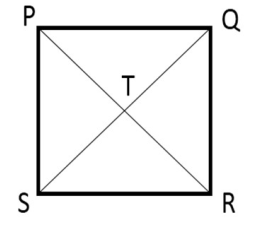
\includegraphics[width=0.2\linewidth]{figs/screenshot003}
	 	\caption{}
	 	\label{fig:screenshot003}
	 	\end{figure}
	 
	 Which one of the following statements is correct as per the information provided above?\\[0.5em]
	  \begin{multicols}{2}
	 \begin{enumerate}[label=(\Alph*)]
	 	\item The sequence of operations (1) and (2) are equivalent
	 	\item The sequence of operations (1) and (3) are equivalent
	 	\item The sequence of operations (2) and (3) are equivalent
	 	\item The sequence of operations (1), (2) and (3) are equivalent
	 \end{enumerate}
	\end{multicols}
	 \hfill (GATE ST 2022)
	 \vspace{2em}
	 \\
Q.11 Let $\mathbf{M}$ be a $2 \times 2$ real matrix such that 
$(\mathbf{I} + \mathbf{M})^{-1} = \mathbf{I} - \alpha \mathbf{M}$, 
where $\alpha$ is a non-zero real number and $\mathbf{I}$ is the $2 \times 2$ identity matrix. 
If the trace of the matrix $\mathbf{M}$ is $3$, then the value of $\alpha$ is:
\begin{multicols}{4}
\begin{enumerate}[label=\alph*.] 
	\item $\frac{3}{4}$
	\item $\frac{1}{3}$
	\item $\frac{1}{2}$
	\item $\frac{1}{4}$
	\end{enumerate}
\end{multicols}
\hfill (GATE ST 2022)\\
	\vspace{2em}
Q.12 Let $ \{X(t)\}_{t\geq0} $ be a linear pure death process with death rate $\mu_i = 5i$, for $i = 0, 1, \dots , N$, where $N \geq 1$. Suppose that $p_i(t) = P(X(t) = i)$. Then the system of forward Kolmogorov equations is:\\

 \begin{enumerate}[label=\alph*.] 
	\item $ \frac{dp_i(t)}{dt} = 5(i + 1)p_{i+1}(t) + 5i p_i(t) \text{ and } \frac{dp_N(t)}{dt} = 5Np_N(t)$ for $i = 0,1, \dots ,N - 1$ with initial conditions $p_i(0) = 0$ for $i \neq N $, and $p_N(0) = 1$.\\
	\item $ \frac{dp_i(t)}{dt} = 5(i + 1)p_{i+1}(t) - 5i p_i(t) \text{ and } \frac{dp_N(t)}{dt} = -5Np_N(t)$ for $i = 0,1, \dots ,N - 1$ with initial conditions $p_i(0) = 0$ for $i \neq N $, and $p_N(0) = 1$.\\
	\item $ \frac{dp_i(t)}{dt} = 5(i + 1)p_{i+1}(t) + 5i p_i(t) \text{ and } \frac{dp_N(t)}{dt} = 5Np_N(t)$ for $i = 0,1, \dots ,N - 1$ with initial conditions $p_i(0) = 1$ for $i \neq N $, and $p_N(0) = 1$.\\
	\item $ \frac{dp_i(t)}{dt} = 5(i + 1)p_{i+1}(t) - 5i p_i(t) \text{ and } \frac{dp_N(t)}{dt} = -5Np_N(t)$ for $i = 0,1, \dots ,N - 1$ with initial conditions $p_i(0) = 0$ for $i \neq N $, and $p_N(0) = 1$.\\
	\hfill (GATE ST 2022)
\end{enumerate}

	\vspace{2em}
Q.13 Let $S^2$ be the variance of a random sample of size $n > 1$ from a normal population with an unknown mean $\mu$ and an unknown finite variance $\sigma^2 > 0$. Consider the following statements:
(I) $S^2$ is an unbiased estimator of $\sigma^2$, and $S$ is an unbiased estimator of $\sigma$.
(II) $(\frac{n-1}{n})S^2$ is a maximum likelihood estimator of $\sigma^2$, and $\sqrt{\frac{n-1}{n}}S$ is a maximum likelihood estimator of $\sigma$.
Which of the above statements is/are true?
\begin{multicols}{4}
\begin{enumerate}[label=\alph*.] 
	\item (I) only
	\item (II) only
	\item Both (I) and (II)
	\item Neither (I) nor (II)
	
\end{enumerate}
\end{multicols}
\hfill (GATE ST 2022)\\
	\vspace{2em}
Q.14 Let $f : \mathbb{R}^2 \to \mathbb{R}$ be a function defined by
\[
f(x,y) =
\begin{cases}
	\dfrac{x^2y}{x^2 + y^2}, & (x,y) \neq (0,0), \\[6pt]
	0, & (x,y) = (0,0).
\end{cases}
\]
Then which one of the following statements is true?
\begin{multicols}{2}
\begin{enumerate}[label=\alph*.] 
	\item $f$ is bounded and $\frac{\partial f}{\partial x}$ is unbounded on $\mathbb{R}^2$.
	\item $f$ is unbounded and $\frac{\partial f}{\partial x}$ is bounded on $\mathbb{R}^2$.
	\item Both $f$ and $\frac{\partial f}{\partial x}$ are unbounded on $\mathbb{R}^2$.
	\item Both $f$ and $\frac{\partial f}{\partial x}$ are bounded on $\mathbb{R}^2$.
	
\end{enumerate}
\end{multicols}
\hfill (GATE ST 2022)\\
	\vspace{2em}
Q.15 Let $X_1, X_2, \dots, X_n$ be a random sample from a distribution with cumulative distribution function $F(x)$. Let the empirical distribution function of the sample be $F_n(x)$. The classical Kolmogorov-Smirnov goodness of fit test statistic is given by
$$ T_n = \sqrt{n}D_n = \sqrt{n} \sup_{-\infty < x < \infty} | F_n(x) - F(x) | $$
Consider the following statements:
(I) The distribution of $T_n$ is the same for all continuous underlying distribution functions $F(x)$.
(II) $D_n$ converges to 0 almost surely, as $n \to \infty$.
Which of the above statements is/are true?
\begin{multicols}{4}
\begin{enumerate}[label=\alph*.] 
	\item (I) only
	\item (II) only
	\item Both (I) and (II)
	\item Neither (I) nor (II)
	
\end{enumerate}
\end{multicols}
\hfill (GATE ST 2022)\\
	\vspace{2em}
Q.16 Consider the following transition matrices $\textbf{P}_1$ and $\textbf{P}_2$ of two Markov chains:
\[
P_1 = 
\begin{bmatrix}
	1 & 0 & 0 \\
	\frac{1}{3} & \frac{1}{2} & \frac{1}{6} \\
	0 & 0 & 1
\end{bmatrix}
\quad \text{and} \quad
P_2 = 
\begin{bmatrix}
	\frac{1}{6} & \frac{1}{3} & \frac{1}{2} \\
	\frac{1}{4} & 0 & \frac{3}{4} \\
	0 & 1 & 0
\end{bmatrix}.
\]
Then which one of the following statements is true?

\begin{enumerate}[label=\alph*.] 
	\item Both $\textbf{P}_1$ and $\textbf{P}_2$ have unique stationary distributions.
	\item $\textbf{P}_1$ has a unique stationary distribution, but $\textbf{P}_2$ has infinitely many stationary distributions.
	\item $\textbf{P}_1$ has infinitely many stationary distributions, but $\textbf{P}_2$ has a unique stationary distribution.
	\item Neither $\textbf{P}_1$ nor $\textbf{P}_2$ has a unique stationary distribution.

\end{enumerate}
	\hfill (GATE ST 2022)\\
	\vspace{2em}
Q.17 Let $\textbf{X}_1, \textbf{X}_2, \dots, \textbf{X}_{20}$ be a random sample of size 20 from $N_6(\mathbf{\mu,\Sigma})$ with $\det(\Sigma) \neq 0$, and suppose both $\mu$ and $\Sigma$ are unknown. Let 
$$
\bar{X} = \frac{1}{20}\sum_{i=1}^{20} X_i 
\quad \text{and} \quad
S = \frac{1}{19} \sum_{i=1}^{20} (X_i - \bar{X})(X_i - \bar{X})^T.
$$ 
Consider the following two statements:
(I) The distribution of $19S$ is $W_6(19,\Sigma)$ (Wishart distribution of order 6 with 19 degrees of freedom).
(II) The distribution of $(X_3 - \mu)^T S^{-1}(X_3 - \mu)$ is $\chi^2_6$ (Chi-square distribution with 6 degrees of freedom).
Then which of the above statements is/are true?
\begin{multicols}{4}
\begin{enumerate}[label=\alph*.] 
	\item (I) only
	\item (II) only
	\item Both (I) and (II)
	\item Neither (I) nor (II)

\end{enumerate}
\end{multicols}
	\hfill (GATE ST 2022)\\
	\vspace{2em}
Q.18 Let $X_1, X_2, \dots, X_{18}$ be a random sample from the distribution
\[
f(x; \theta) =
\begin{cases}
	\dfrac{2x}{\theta} e^{-x^2/\theta}, & x > 0, \\[4pt]
	0, & x \leq 0.
\end{cases}
\]
Let $\chi^2_{\alpha,n}$ denote the value of a Chi-square random variable Y with n degrees of freedom such that $P(Y > \chi^2_{\alpha, n}) = \alpha$. If $x_1, x_2, \dots, x_{18}$ is a realization of this random sample, then, based on the sufficient statistic $\sum_{i = 1}^{18} X^2_i$, which one of the following is a 98\% confidence interval for $\theta$?
 \begin{multicols}{4}
\begin{enumerate}
	\item $	\left( 
	\dfrac{2 \sum_{i=1}^{18} x_i^2}{\chi^2_{0.01,36}},\;
	\dfrac{2 \sum_{i=1}^{18} x_i^2}{\chi^2_{0.99,36}} 
	\right)
	$
	\item	$
	\left( 
	\dfrac{2 \sum_{i=1}^{18} x_i^2}{\chi^2_{0.01,18}},\;
	\dfrac{2 \sum_{i=1}^{18} x_i^2}{\chi^2_{0.99,18}} 
	\right)$
	\item$ 	\left( 
	\dfrac{ \sum_{i=1}^{18} x_i^2}{\chi^2_{0.01,36}},\;
	\dfrac{ \sum_{i=1}^{18} x_i^2}{\chi^2_{0.99,36}} 
	\right)$
	\item $	\left( 
	\dfrac{\sum_{i=1}^{18} x_i^2}{\chi^2_{0.01,18}},\;
	\dfrac{\sum_{i=1}^{18} x_i^2}{\chi^2_{0.99,18}} 
	\right)$

\end{enumerate}
\end{multicols}
	\hfill (GATE ST 2022)\\
	\vspace{2em}
Q.19 Let $X_1,X_2, \dots ,X_n$ be a random sample from a population $f(\chi; \theta)$ , where $\theta$ is a parameter .Then which one of the follwoing statements is NOT true ?\\
(A) $\sum_{i=1}^{n}$ $X_i$ is a complete and sufficient  statistic for $\theta$, if \[
f(x; \theta) = 
\dfrac{e^{-\theta}\,\theta^{x}}{x!} , x = 0,1,2, ..., and \theta > 0
\]\\

\begin{enumerate}
	\item[(B)] 
	$(\sum_{i=1}^n X_i,\; \sum_{i=1}^n X_i^2)$ is a complete and sufficient statistic for $\theta$, if 
	\[
	f(x; \theta) = \frac{1}{\sqrt{2 \pi}\,\theta}\,
	e^{-\frac{1}{2\theta^2}(x-\theta)^2},
	\quad -\infty < x < \infty,\; \theta > 0
	\]
	\item[(C)] 
	$f(x; \theta) = \theta x^{\theta - 1},\; 0 < x < 1,\; \theta > 0$
	has monotone likelihood ratio property in 
	$
	\prod_{i=1}^{n} X_i
	$
	\\
	\item[(D)] 
	$X_{(n)} - X_{(1)}$ is ancillary statistic for $\theta$ if 
	$f(x;\theta)=1,\; 0 < \theta < x < \theta+1$, where 
	\[
	X_{(1)} = \min\{X_1, X_2, \ldots, X_n\}, 
	\quad 
	X_{(n)} = \max\{X_1, X_2, \ldots, X_n\}
	\]
	\end{enumerate}
\hfill (GATE ST 2022)\\
Q.20 A random sample $X_1,X_2, \dots, X_6$ of size 6 is taken from a Bernoulli distribution with
the parameter $\theta$. The null hypothesis $H_o$ : $\theta = \frac{1}{2}$ is to be tested against the alternative hypothesis $H_1 : \theta > \frac{1}{2}$ ,based on the statistic Y = $\sum_{i=6}^{6}X_i$.If the value of Y
corresponding to the observed sample values is 4, then the p-value of the test
statistic is 
\\
\begin{multicols}{4}
(A) $\frac{21}{32}$\\
(B) $\frac{9}{64}$\\
(C) $\frac{11}{32}$\\
(D) $\frac{7}{64}$\\
\end{multicols}
\hfill (GATE ST 2022)\\
Q.21 Let $\{a_n\}_{n=1}^{\infty}$ be a sequence of positive real numbers satisfying 
\[
\frac{8}{a_{n+1}} = \frac{7}{a_n} + \frac{a_n^2}{343}, 
\qquad n \geq 1
\]
with $a_1 = 3$ and $a_n < 7$ for all $n \geq 2$. 

Consider the following statements:

\begin{enumerate}
	\item[(I)] $\{a_n\}$ is monotonically increasing.
	\item[(II)] $\{a_n\}$ converges to a value in the interval $[3,7]$.
\end{enumerate}


Then which of the above statements is/are true?\\
\begin{multicols}{4}
(a) (I) only \\
(b) (II) only \\
(c) Both (I) and (II)\\
(d) Neither (I) nor (II)
\end{multicols}
 \hfill (GATE ST 2022)\\
 \\
Q.22 Let \textbf{M} be any squar e matrix of arbitrary order n such that $\textbf{M}^2$  = \textbf{0} AND THE NULLITY OF m IS 6.Then the maximum possible value of n \textbf{(in integer)} is \underline{\hspace{2cm}}.\hfill (GATE ST 2022)\\
\\
\\
	\vspace{2em}
Q.23 Consider the usual inner product in \textbf{Q.23} Consider the usual inner product in $\mathbb{R}^4$. 
Let $\mathbf{u} \in \mathbb{R}^4$ be a unit vector orthogonal to the subspace
\[
S = \{ (x_1, x_2, x_3, x_4)^T \in \mathbb{R}^4 
\mid x_1 + x_2 + x_3 + x_4 = 0 \}.
\]
If $\mathbf{v} = (1, -2, 1, 1)^T$, and the vectors $\mathbf{u}$ and 
$\mathbf{v} - \alpha \mathbf{u}$, $\alpha \in \mathbb{R}$, are orthogonal, 
then the value of $\alpha^2$ (\textit{rounded off to two decimal places}) is equal to 
\underline{\hspace{2cm}}. \hfill (GATE ST 2022)\\
\\
\\
Q.24 Let $\{ B(t) \}_{t \geq 0}$ be a standard Brownian motion and let 
$\Phi(\cdot)$ be the cumulative distribution function of the standard normal distribution. 
If 
\[
P\big( (B(2) + 2B(3)) > 1 \big)
= 1 - \Phi\left( \frac{1}{\sqrt{\alpha}} \right), 
\qquad \alpha > 0,
\]
then the value of $\alpha$ (in integer) is equal to 
\underline{\hspace{2cm}}. \hfill (GATE ST 2022)\\
\\
\\
Q.25 Let X and Y be two independent exponential random variables with $E(X^2) = \frac{1}{2} $ and $E(Y^2)$ = $\frac{2}{9}$ .Then p($ X < 2Y$) \textbf{(rounded off to to decimal places)} is equal to \underline{\hspace{2cm}}. \hfill (GATE ST 2022)\\
\\
\\
Q.26 Let X be a random variable with the probability mass function $p_x(x) = (\frac{3}{4})^{x-1}\frac{1}{4}$ ,x = 1,2,3, \dots. Then the value of \[ \sum_{n=0}^{\infty}P(n < X \leq n + 3)
\]
\textbf{(rounded off to two decimal places)} is equal to \underline{\hspace{2cm}} . \hfill (GATE ST 2022)\\
\\
\\
Let $X_i, \; i = 1, 2, \ldots, n,$ be i.i.d. random variables from a normal distribution 
with mean $1$ and variance $4$. Let 
\[
S_n = X_1^2 + X_2^2 + \cdots + X_n^2.
\]
If $\mathrm{Var}(S_n)$ denotes the variance of $S_n$, then the value of
\[
\lim_{n \to \infty} 
\left(
\frac{\mathrm{Var}(S_n)}{n} 
- 
\left(\frac{\mathbb{E}(S_n)}{n}\right)^2
\right)
\]
\textbf{(in integer)} is equal to \underline{\hspace{2cm}} .\hfill (GATE ST 2022)\\
\\
\\
Q.28 At a telephone exchange, telephone calls arrive independently at an average rate of
1 call per minute, and the number of telephone calls follows a Poisson distribution.
Five time intervals, each of duration 2 minutes, are chosen at random. Let p denote
the probability that in each of the five time intervals at most 1 call arrives at the
telephone exchange. Then $e^{10}p$(in integer is equal to \underline{\hspace{2cm}}.\hfill (GATE ST 2022)\\
\\
\\
Q.29 Let X be a random variable with the probability density function.\\
\[ 
f(x) = \begin{cases}
	c(x - [x]), &  0 < x < 3 \\
	0, & elsewhere,\\
	\end{cases}
\]
where C is a constant and [x] denotes the greatest integer less than or equal to x.If $A = [\frac{1}{2},2]$, then P(X $\in$ A) (\textbf{rounded off to two decimal  places}) is equal to \underline{\hspace{2cm}}.\hfill (GATE ST 2022)\\
\\
\\
Q.30 Let X and Y be two random variables such that the moment generating function of X is M(t) and the moment generating function of Y is \[
H(t) = \left( \frac{3}{4} e^{2t} + \frac{1}{4} \right) M(t),
\]
where $t \in (-h,h),\, h > 0$. If the mean and the variance of $X$ are $\frac{1}{2}$ and $\frac{1}{4}$, respectively, then the variance of $Y$ \textbf{(in integer)} is equal to \underline{\hspace{2cm}}.\hfill (GATE ST 2022)\\
\\
\\
Q.31 Let $X_i, \, i = 1, 2, \ldots, n,$ be \textit{i.i.d.} random variables with the probability density function
\[
f_X(x) = 
\begin{cases} 
	\frac{1}{\sqrt{2}\,\Gamma\left(\frac{1}{6}\right)} x^{-5/6} e^{-x/8}, & 0 < x < \infty, \\
	0, & \text{elsewhere},
\end{cases}
\]
where $\Gamma(\cdot)$ denotes the gamma function. Also, let $\overline{X}_n = \frac{1}{n}(X_1 + X_2 + \cdots + X_n)$. If
$
\sqrt{n} \left( \overline{X}_n \left(3 - \overline{X}_n \right) - \frac{20}{9} \right)
$
converges to $\mathrm{N}(0, \sigma^2)$ in distribution, then $\sigma^2$ \textbf{(rounded off to two decimal places)} is equal to \underline{\hspace{2cm}} .\hfill (GATE ST 2022)\\
\\
\\
Q.32 Consider a Poisson process $\{X(t), t \geq 0\}$. The probability mass function of $X(t)$ is given by
\[
f(t) = \frac{e^{-4t} (4t)^n}{n!}, \quad n=0,1,2,\dots
\]
If $C(t_1,t_2)$ is the covariance function of the Poisson process, then the value of $C(5,3)$ is equal to \underline{\hspace{2cm}}.\hfill (GATE ST 2022)\\
\\
\\
Q.33 A random sample of size 4 is taken from the distribution with the probability density
function $
f(x; \theta) = \begin{cases}
	\frac{2(\theta - x)}{\theta^2}, & 0 < x < \theta \\
	0, & elsewhere,
\end{cases}
$
\\
\\
If the observed sample values are 6, 5, 3, 6, then the method of moments estimate (in integer) of the parameter $\theta$,based on these observations, is \underline{\hspace{2cm}}.\hfill (GATE ST 2022)\\
\\
\\
Q.34 A company sometimes stops payments of quarterly dividends. If the company pays the quarterly dividend, the probability that the next one will be paid is 0.7. If the  company stops the quarterly dividend, the probability that the next quarterly dividend will not be paid is 0.5. Then the probability (rounded off to three decimal places) that the company will not pay quarterly dividend in the long run is \underline{\hspace{2cm}}. \hfill (GATE ST 2022)\\
\\
\\
Q.35 Let $X_1,X_2, \dots,X_8$ be a random sample taken from a distribution funnction of the sample. If $\alpha$ is the variance of $F_8(2)$,then 128$\alpha$ (in integer) is equal to \underline{\hspace{2cm}.}\hfill (GATE ST 2022)\\
\\
\pagebreak
\\
\fbox{\textbf{Q.36 – Q.65 Carry TWO marks Each}}\\
\\
Q.36 Let \textbf{M} be a 3 x 3 real symmetric matrix with eigenvalues -1, 1, 2 and the corresponding unit eigenvectors \textbf{u, v, w}, respectively. Let \textbf{x} and \textbf{y} be two vectors in $\mathbb{R}^3$ such that
\[
\mathbf{M} \mathbf{x} = \mathbf{u} + 2(\mathbf{v} + \mathbf{w}) \hspace{1cm} \text{and} \hspace{1cm} \mathbf{M}^2\mathbf{y} = \mathbf{u} -(\mathbf{v} + 2\mathbf{w})
\]
Considering the usual inner product in $\mathbb{R}^3$, the value of ${|\mathbf{x} + \mathbf{y}|}^2$, where $|\mathbf{x} + \mathbf{y}|$ is the length of the vector $\mathbf{x + y}$, is
\begin{multicols}{4}
\begin{enumerate}[label=\Alph*.] 
	\item 1.25
	\item 0.25
	\item 0.75
	\item 1

\end{enumerate}
\end{multicols}
\hfill (GATE ST 2022)\\
	\vspace{2em}
Q.37 Consider the following infinite series:
\[
S_1 := \sum_{n=0}^{\infty} (-1)^n \frac{n}{n^2 + 4} \quad \text{and} \quad 
S_2 := \sum_{n=0}^{\infty} (-1)^n \left(\sqrt{n^2 + 1} - n \right).
\]
Which of the above series is/are conditionally convergent?
\begin{multicols}{4}
\begin{enumerate}[label=\Alph*.] 
	\item $S_1$ only
	\item $S_2$ only
	\item Both $S_1$ and $S_2$
	\item Neither $S_1$ nor $S_2$

\end{enumerate}
\end{multicols}
\hfill (GATE ST 2022)\\
	\vspace{2em}
Q.38 Let ${(3,6)}^T$, ${(4,4)}^T$, ${(5,7)}^T$ and ${(4,7)}^T$ be four independent observations from a bivariate normal distribution with the mean vector $\mathbf{\mu}$ and the covariance matrix $\mathbf{\Sigma}$. Let $\hat{\mu}$ and $\hat{\Sigma}$ be the maximum likelihood estimates of $\mu$ and $\Sigma$, respectively, based on these observations. Then $\hat{\mu}$ is equal to 
\begin{multicols}{4}
\begin{enumerate}[label=\Alph*.] 
	\item $\begin{pmatrix} 3.5\\ 6.0 \end{pmatrix}$
	\item $\begin{pmatrix} 4.0\\ 6.0 \end{pmatrix}$
	\item $\begin{pmatrix} 4.0\\ 13.5 \end{pmatrix}$
	\item $\begin{pmatrix} 16.0\\ 24.0 \end{pmatrix}$

\end{enumerate}
\end{multicols}
\hfill (GATE ST 2022)\\
	\vspace{2em}
Q.39 Let 
$
\mathbf{X} = \begin{pmatrix} X_1 \\ X_2 \\ X_3 \end{pmatrix}
$
follow 
$
N_3(\mu, \Sigma)
$
with 
$
\mu = \begin{pmatrix} 2 \\ -3 \\ 2 \end{pmatrix}
\quad \text{and} \quad
\Sigma = \begin{bmatrix}
	4 & -1 & 1 \\
	-1 & 2 & a \\
	1 & a & 2
\end{bmatrix},
$
where \(a \in \mathbb{R}\). Suppose that the partial correlation coefficient between \(X_2\) and \(X_3\), keeping \(X_1\) fixed, is \(\frac{5}{7}\). Then a is equal to
\begin{multicols}{4}
\begin{enumerate}[label=\Alph*.] 
	\item 1
	\item $\frac{3}{2}$
	\item 2
	\item $\frac{1}{2}$

\end{enumerate}
\end{multicols}
\hfill (GATE ST 2022)\\
	\vspace{2em}
Q.40 If the line y = $\alpha$x, $\alpha \geq \sqrt{2}$, divides the area of the region 
\[
R:= \{(x,y) \in \mathbb{R}^2|0 \leq x \leq \sqrt{y}, 0 \leq y \leq 2\}
\]
into two equal parts, then the value of $\alpha$ is equal to
\begin{multicols}{4}
\begin{enumerate}[label=\alph*.] 
	\item $\frac{3}{\sqrt{2}}$
	\item $2\sqrt{2}$
	\item $\sqrt{2}$
	\item $\frac{5}{2\sqrt{2}}$

\end{enumerate}
\end{multicols}
\hfill (GATE ST 2022)\\
	\vspace{2em}
Q.41 Let (X,Y,Z) be a random vector with the joint probability density function
\[
f_{X,Y,Z}(x,y,z) = 
\begin{cases}
	\frac{1}{3} (2x + 3y + z), & 0 < x < 1,\, 0 < y < 1,\, 0 < z < 1, \\
	0, & \text{elsewhere}.
\end{cases}
\]
Then which one of the following points is on the regression surface of X on (Y,Z)?
\begin{multicols}{4}
\begin{enumerate}[label=\Alph*.] 
	\item $( \frac{4}{7}, \frac{1}{3}, \frac{1}{3} )$
	\item $( \frac{6}{7}, \frac{2}{3}, \frac{2}{3} )$
	\item $(\frac{1}{2},\frac{1}{3},\frac{2}{3})$
	\item $(\frac{1}{2},\frac{2}{3},\frac{1}{3})$
	
\end{enumerate}
\end{multicols}
\hfill (GATE ST 2022)\\
	\vspace{2em}
Q.42 A random sample X of size one is taken from a distribution with the probability density function \[
f(x; \theta) = \begin{cases}
	\frac{2x}{\theta^2}, & 0 < x < \theta \\
	0, & \text{elsewhere},
\end{cases}
\]
if $\frac{X}{\theta}$ is used as a pivot for obtaining the confidence interval for $\theta$, then which one of the following is an 80\% confidence interval (confidence limits rounded off to three decimal places) for $\theta$ based on the observed sample value x = 10?
\begin{multicols}{4}
\begin{enumerate}[label=\Alph*.] 
	\item (10.541, 31.623)
	\item (10.987, 31.126)
	\item (11.345, 30.524)
	\item (11.267, 30.542)

\end{enumerate}
\end{multicols}
\hfill (GATE ST 2022)\\
	\vspace{2em}
Q.43 Let \(X_1, X_2, \ldots, X_7\) be a random sample from a normal population with mean 0 and variance \(\theta > 0\). Let
\[
K = \frac{X_1^2 + X_2^2}{X_1^2 + X_2^2 + \cdots + X_7^2}.
\]
Consider the following statements:
\begin{enumerate}[label=\Alph*.] 
	\item[(I)] The statistics \(K\) and \(X_1^2 + X_2^2 + \cdots + X_7^2\) are independent.
	\item[(II)] \(\frac{7K}{2}\) has an \(F\)-distribution with 2 and 7 degrees of freedom.
	\item[(III)] \(E(K^2) = \frac{8}{63}.\)
\end{enumerate}
Then which of the above statements is/are true?
\begin{multicols}{4}
\begin{enumerate}[label=\Alph*.] 
	\item (I) and (II) only
	\item (I) and (III) only
	\item (II) and (III) only
	\item (I) only

\end{enumerate}
\end{multicols}
\hfill (GATE ST 2022)\\
	\vspace{2em}
Q.44 Consider the following statements :\\
(I) Let a random variable X have the probability density function 
\[
f_X(x) = \frac{1}{2}e^{-|x|}, \hspace{1cm} -\infty < x < \infty.
\]
Then there exist i.i.d. random variables $X_1$ and $X_2$ such that X and $X_1 - X_2$ have the same distribution. \\
(II) Let a random variable Y have the probability density function 
\[
f_Y(y) = \begin{cases}
	\frac{1}{4}, & -2 < y < 2,\\
	0, & \text{elsewhere}.
\end{cases}
\]
Then there exist i.i.d. random variables $Y_1$ and $Y_2$ such that Y and $Y_1 - Y_2$ have the same distribution.\\
Then which of the above statements is/are true?
\begin{multicols}{4}
\begin{enumerate}[label=\Alph*.] 
	\item (I) only
	\item (II) only
	\item both (I) and (II)
	\item Neither (I) nor (II)

\end{enumerate}
\end{multicols}
\hfill (GATE ST 2022)\\
	\vspace{2em}
Q.45 Suppose \(X_1, X_2, \ldots, X_n, \ldots\) are independent exponential random variables with the mean \(\frac{1}{2}\). Let the notation \emph{i.o.} denote "infinitely often". Then which of the following is/are true?
\begin{multicols}{2}
\begin{enumerate}[label=\alph*.] 
	\item P(\{$x_n > \frac{\epsilon}{2}\log_en$\} i.o.) = 1 for $0 < \epsilon \leq 1$
	\item P(\{$x_n < \frac{\epsilon}{2}\log_en$\} i.o.) = 1 for $0 < \epsilon \leq 1$
	\item P(\{$x_n > \frac{\epsilon}{2}\log_en$\} i.o.) = 1 for $\epsilon > 1$
	\item P(\{$x_n < \frac{\epsilon}{2}\log_en$\} i.o.) = 1 for $\epsilon > 1$

\end{enumerate}
\end{multicols}
\hfill (GATE ST 2022)\\
	\vspace{2em}
Q.46 Let \(\{X_n\}, n \ge 1\), be a sequence of random variables with the probability mass functions
\[
p_{X_n}(x) = 
\begin{cases}
	\frac{n}{n+1}, & x = 0, \\[6pt]
	\frac{1}{n+1}, & x = n, \\[6pt]
	0, & \text{elsewhere}.
\end{cases}
\]
Let \(X\) be a random variable with \(P(X=0)=1\). Then which of the following statements is/are true?

\begin{enumerate}[label=\Alph*.] 
	\item \(X_n\) converges to \(X\) in distribution.
	\item \(X_n\) converges to \(X\) in probability.
	\item \(E(X_n) \longrightarrow E(X)\).
	\item There exists a subsequence \(\{X_{n_k}\}\) of \(\{X_n\}\) such that \(X_{n_k}\) converges to \(X\) almost surely.
\end{enumerate}
\hfill (GATE ST 2022)\\
\vspace{2em}
Q.47 5Let \textbf{M} be any 3 × 3 symmetric matrix with eigenvalues 1, 2 and 3. Let \textbf{N} be any 3 × 3 matrix with real eigenvalues such that \textbf{MN} + \textbf{NM} = 3\textbf{I}, where \textbf{I} is the 3 × 3 identity matrix. Then which of the following cannot be eigenvalue(s) of the matrix \textbf{N}?
\begin{multicols}{4}
\begin{enumerate}[label=\Alph*.] 
	\item $\frac{1}{4}$ 
	\item $\frac{3}{4}$
	\item $\frac{1}{2}$
	\item $\frac{7}{4}$

\end{enumerate}
\end{multicols}
\hfill (GATE ST 2022)\\
	\vspace{2em}
Q.48 Let \(M\) be a \(3 \times 2\) real matrix having a singular value decomposition as $M = USV^T,$ where the matrix $
S = \begin{bmatrix}
	\sqrt{3} & 0 \\
	0 & 1 \\
	0 & 0
\end{bmatrix},
$
\(U\) is a \(3 \times 3\) orthogonal matrix, and \(V\) is a \(2 \times 2\) orthogonal matrix. Then which of the following statements is/are true?
\begin{enumerate}[label=\Alph*.] 
	\item The rank of the matrix \(M\) is 1.
	\item The trace of the matrix \(M^TM\) is 4.
	\item The largest singular value of the matrix \((M^TM)^{-1}M^T\) is 1.
	\item The nullity of the matrix \(M\) is 1.
\end{enumerate}
\hfill (GATE ST 2022)\\
	\vspace{2em}
Q.49 Let X be a random variable such that 
\[
P\left(\frac{a}{2\pi}X \in \mathbb{Z}\right) = 1, \hspace{1cm} a > 0.
\]
Then which of the following statements is/are true?
\begin{multicols}{2}
\begin{enumerate}[label=\Alph*.] 
	\item $\phi_X(a) = 1$
	\item $\phi_X(.)$ is periodic with period a.
	\item $|\phi_X(t)| < 1$ for all $t \neq a$.
	\item $\int_{0}^{2\pi} e^{itn} \phi_X(t) dt = \pi P\left(X = \frac{2\pi n}{a}\right), n \in \mathbb{Z}, i = \sqrt{-1}$
\end{enumerate}
\end{multicols}
\hfill (GATE ST 2022)\\
Q.50 Which of the following real valued functions is/are uniformly continuous on $[0, \infty)$?
\begin{multicols}{4}
\begin{enumerate}[label=\Alph*.] 
	\item $\sin^2 x$
	\item $x \sin x$
	\item $\sin(\sin x)$
	\item $\sin(x \sin x)$
	
\end{enumerate}
\end{multicols}
\hfill (GATE ST 2022)\\
	\vspace{2em}
Q.51 Two independent random samples, each of size 7, from two populations yield the following values:
\[
\begin{tabular}{|c|c|c|c|c|c|c|c|}
	\hline
	Population 1 & 18 & 20 & 16 & 20 & 17 & 18 & 14 \\
	\hline
	Population 2 & 17 & 18 & 14 & 20 & 14 & 13 & 16 \\
	\hline
\end{tabular} 
\]
If Mann-Whitney U test is performed at 5\% level of significance to test the null hypothesis $H_0$: Distributions of the populations are same, against the alternative hypothesis $H_1$: Distributions of the populations are not same, then the value of the test statistic U (in integer) for the given data, is \underline{\hspace{2cm}}.\hfill (GATE ST 2022)\\
\\
\\
Q.52 Consider the multiple regression model
\[
Y = \beta_0 + \beta_1X_1 + \beta_2X_2 + \beta_3X_3 + \epsilon
\]
where $\epsilon$ is normally distributed with mean 0 and variance $\sigma^2 > 0$ and $\beta_0, \beta_1, \beta_2, \beta_3$ are unknown parameters. Suppose 52 observations of ($Y, X_1, X_2, X_3$) yield sum of squares due to regression as 18.6 and total sum of squares as 79.23. Then, for testing the null hypothesis $H_0: \beta_1 = \beta_2 = \beta_3 = 0$ against the alternative hypothesis $H_1: \beta_i \neq 0$ for some $i = 1, 2, 3$, the value of the test statistic \textbf{(rounded off to three decimal places)}, based on one way analysis of variance, is \underline{\hspace{2cm}}.\hfill (GATE ST 2022)\\
\\
\\
Q.53 Suppose a random sample of size 3 is taken from a distribution with the probability density function 
\[
f(x) = \begin{cases}
	2x, & 0 < x < 1, \\
	0, & \text{elsewhere},
\end{cases}
\]
If P is the probability that the largest sample observation is at least twice the smallest sample observation, then the value of P \textbf{(rounded off to three decimal places)} is \underline{\hspace{2cm}}.\hfill (GATE ST 2022)\\
\\
\\
Q.54 Let a linear model Y = $\beta_0 + \beta_1X + \epsilon$ be fitted to the following data, where $\epsilon$ is normally distributed with mean 0 and unknown variance $\sigma^2 > 0$. 
\[
\begin{tabular}{|c|c|c|c|c|c|}
	\hline
	$x_i$ & 0 & 1 & 2 & 3 & 4 \\
	\hline
	$y_i$ & 3 & 4 & 5 & 6 & 7 \\
	\hline
\end{tabular}
\]
Let $\hat{Y}$ denote the ordinary least-square estimator of Y at X = 6, and the variance of $\hat{Y} = c\sigma^2$. Then the value of the real constant c \textbf{(rounded off to one decimal place)} is equal to \underline{\hspace{2cm}}.\hfill (GATE ST 2022)\\
\\
\\
Q.55 Let 0, 1, 1, 2, 0 be five observations of a random variable X which follows a Poisson distribution with the parameter $\theta > 0$. Let the minimum variance unbiased estimate of P(X $\leq$ 1), based on this data, be $\alpha$. Then 5$\alpha$ \textbf{(in integer)} is equal to \underline{\hspace{2cm}}.\hfill (GATE ST 2022)\\
\\
\\
Q.56 While calculating Spearman’s rank correlation coefficient, based on n observations $\{(x_i , y_i), i = 1, 2, \dots, n\}$ from a paired data, it is found that $x_i$ are distinct for all $i \ge 2$, $x_1 = x_2$ and $\sum_{i=1}^{n}d^2_i = 19.5$, where $d_i = \text{rank}(x_i) - \text{rank}(y_i)$. Then the minimum possible value of $n^3 - n$ \textbf{(in integer)} is \underline{\hspace{2cm}}.\hfill (GATE ST 2022)\\
\\
\\
Q.57 In a laboratory experiment, the behavior of cats are studied for a particular food preference between two foods A and B. For an experiment, 70\% of the cats that had food A will prefer food A, and 50\% of the cats that had food B will prefer food A. The experiment is repeated under identical conditions. If 40\% of the cats had food A in the first experiment, then the percentage (rounded off to one decimal place) of cats those will prefer food A in the third experiment, is \underline{\hspace{2cm}}.\hfill (GATE ST 2022)\\
\\
\\
Q.58 A random sample of size 5 is taken from a distribution with the probability density function
\[
f(x; \theta) =
\begin{cases}
	\frac{3x^2}{\theta^3}, & 0 < x < \theta, \\
	0, & \text{elsewhere},
\end{cases}
\]
where $\theta$ is an unknown parameter. If the observed values of the random sample are 3, 6, 4, 7, 5, then the maximum likelihood estimate of the $\frac{1}{8}$th quantile of the distribution \textbf{(rounded off to one decimal place)} is \underline{\hspace{2cm}}.\hfill (GATE ST 2022)\\
\\
\\
Q.59 Consider a gamma distribution with the probability density function 
\[
f(x; \beta) = \begin{cases}
	\frac{1}{24\beta^5}x^4 e^{-x/\beta}, & x > 0,\\
	0, & \text{elsewhere},
\end{cases}
\]
with $\beta > 0$. Then, for $\beta = 2$, the value of the Cramer-Rao lower bound (\textbf{rounded off to one decimal place}) for the variance of any unbiased estimator of $\beta^2$, based on a random sample of size 8 from this distribution, is \underline{\hspace{2cm}}.\hfill (GATE ST 2022)\\
\\
\\
Q.60 Let $X_1, X_2, X_3, X_4$ be a random sample of size four from a Bernoulli distribution with the parameter $\theta$, $0 < \theta < 1$. Consider the null hypothesis $H_0: \theta = \frac{1}{4}$ against the alternative hypothesis $H_1: \theta > \frac{1}{4}$. Suppose $H_0$ is rejected if and only if $X_1 + X_2 + X_3 + X_4 > 2$. If $\alpha$ is the probability of Type I error for the test and $\gamma(\theta)$ is the power function of the test, then the value of $16\alpha + 7 \gamma \left(\frac{1}{2}\right)$ \textbf{(in integer)} is equal to \underline{\hspace{5cm}}.\hfill (GATE ST 2022)\\
\\
\\
Q.61 Given that $\Phi(1.645) = 0.95$ and $\Phi(2.33) = 0.99$, where $\Phi(\cdot)$ denotes the cumulative distribution function of a standard normal random variable. For a random sample $X_1, X_2, \dots, X_n$ from a normal population $N(\mu, \sigma^2)$, where $\mu$ is unknown, the null hypothesis $H_0: \mu = 10$ is to be tested against the alternative hypothesis $H_1: \mu = 12$. Suppose that a test that rejects $H_0$ if the sample mean $\bar{X}$ is large, is used. Then the smallest value of \textbf{n} (in integer) such that Type I error is at most 0.05 and Type II error is at most 0.01, is \underline{\hspace{2cm}}.\hfill (GATE ST 2022)\\
\\
\\
Q.62 Let $Y_1 < Y_2 < \dots < Y_n$ be the order statistics of a random sample of size n from a continuous distribution, which is symmetric about its mean $\mu$. Then the smallest value of n (in integer) such that $P(Y_1 < \mu < Y_n) \geq 0.99$, is \underline{\hspace{2cm}}.\hfill (GATE ST 2022)\\
\\
\\
Q.63 If P(x, y, z) is a point which is nearest to the origin and lies on the intersection of the surfaces $z = xy + 5$ and $x + y + z = 1$. Then the distance (in integer) between the origin and the point P is \underline{\hspace{2cm}}.\hfill (GATE ST 2022)\\
\\
\\
Q.64 Let X and Y be random variables such that X is uniformly distributed over (0, 4), and the conditional distribution of Y given X = x is uniformly distributed over $(0, \frac{x^2}{4})$. Then E($Y^2$) (\textbf{rounded-off to three decimal places}) is equal to \underline{\hspace{2cm}}.\hfill (GATE ST 2022)\\
\\
\\
Q.65 Let X = $(X_1, X_2, X_3)^T$ be a random vector with the distribution $N_3(\mu, \Sigma)$, where 
\[
\mu = \begin{pmatrix}
	3 \\
	2 \\
	4\\
\end{pmatrix}
\hspace{1cm} \text{and} \hspace{1cm} \Sigma = \begin{bmatrix}
	4 & 2 & 1 \\
	2 & 3 & 0 \\
	1 & 0 & 2 \\
\end{bmatrix}.
\]
Then $E(X_1|X_2 = 4, X_3 = 7)$ (\textbf{in integer}) is equal to \underline{\hspace{2cm}}.\hfill (GATE ST 2022)
	

\end{document}

